\documentclass[parskip=full]{scrartcl}
\usepackage[utf8]{inputenc} % use utf8 file encoding for TeX sources 

\usepackage[T1]{fontenc} % avoid garbled Unicode text in pdf 
\usepackage[german]{babel} % german hyphenation, quotes, etc 
\usepackage{hyperref} % detailed hyperlink/pdf configuration
\usepackage{graphicx}
\usepackage[toc]{glossaries}
\usepackage{caption}
\usepackage{pdfpages}
\hypersetup{ % ‘texdoc hyperref‘ for options 
	pdftitle={Entwurf}, %
	bookmarks=true,%
}
\usepackage{csquotes} % provides \enquote{} macro for "quotes"
\usepackage{enumitem}
\makeglossaries



\newglossaryentry{FCM}
{
	name={FCM},
	description={Firebase Cloud Messaging \href{https://firebase.google.com/docs/cloud-messaging/}{https://firebase.google.com/docs/cloud-messaging/}},
	first={Firebase Cloud Messaging(FCM)},
	long={Firebase Cloud Messaging}
}
\begin{document}
	\section{Einleitung}
		bli bla blub
	\section{Klassendiagramme}
		\subsection{Spiel}
		\newpage
		\subsection{GUI}
		\newpage
		\subsection{Server}
		\begin{minipage}{\linewidth}
			\centering
			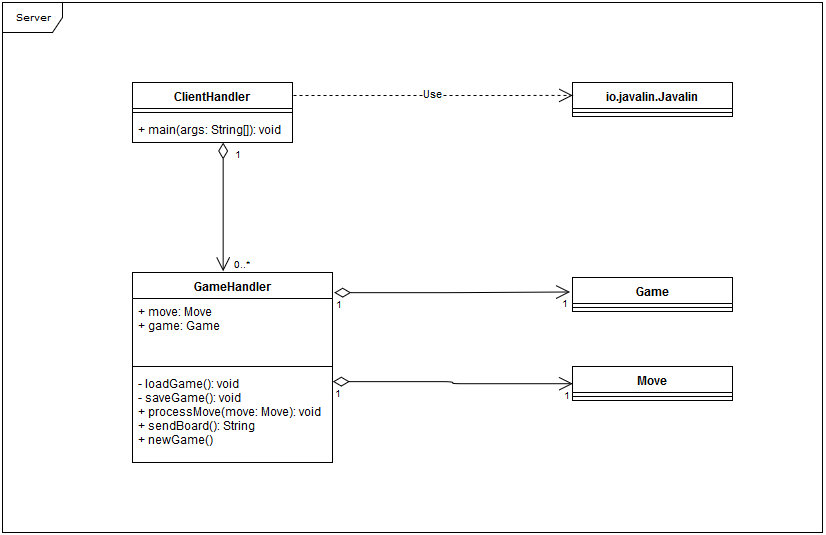
\includegraphics[width=1\linewidth]{Diagramme/Server}
			\captionof{figure}{Server}
			\label{fig:server}
		\end{minipage}
		\begin{itemize}
			\item \textbf{ClientHandler}
			\begin{description}
				\item \textbf{\textit{main(String[] args):}}
				Die main Methode des Servers. Hier wird der Javalin Server gestartet und für jede Anfrage ein neues GameHandler Objekt erzeugt. Diesem werden die gesendeten Anfragen übermittelt. 
			\end{description} 
	
	
			\item \textbf{GameHandler}
			\begin{description}
				\item \textbf{\textit{Move move:}}
				Der Zug, den der GameHandler übermittelt bekommen hat.
				\item \textbf{\textit{Game game:}}
				Das Spiel, das aus der Datenbank geladen wurde.
				\item \textbf{\textit{loadGame():}}
				Lädt das aktuelle Spiel des Spielers aus der Datenbank und erzeugt daraus ein Game Objekt.
				\item \textbf{\textit{saveGame():}}
				Speichert das Game Objekt wieder als String in der Datenbank ab.
				\item \textbf{\textit{processMove():}}
				Führt zuerst loadGame() aus, überprüft den gegebenen Zug auf Gültigkeit, wendet diesen an, sendet ihn an den anderen Spieler und führt anschließend saveGame() aus.
				\item \textbf{\textit{sendBoard():}}
				Sendet das Brett des Spiels per \gls{FCM}.
				\item \textbf{\textit{sendMove():}}
				Übermittelt den Zug per \gls{FCM} an den anderen Spieler.
			\end{description} 
		\end{itemize}
	\section{Sequenzdiagramm}
\printglossaries
\end{document}